\documentclass[18pt,a4paper]{extarticle}
\usepackage[utf8]{inputenc}
\usepackage{amsmath}
\usepackage{amsfonts}
\usepackage{amssymb}
\usepackage{graphicx}
\usepackage{booktabs}
\usepackage{listings}
\usepackage{hyperref}
\usepackage{siunitx}
\usepackage{url}

\author{Frank Hermann}
\title{Radar code documentation}

\DeclareMathOperator{\sgn}{sgn}
\DeclareMathOperator{\Cov}{Cov}
\renewcommand{\Re}{\mathrm{Re}}
\renewcommand{\d}[1]{\ensuremath{\operatorname{d}\!{#1}}}
\setlength\parindent{0pt}

\begin{document}
\maketitle
\begin{figure}
	\centering
	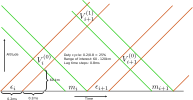
\includegraphics[width=1\linewidth]{code_diagram.pdf}
	\caption{Range time diagram of the simplified version of the radar code.}
	\label{fig:sketch}
\end{figure}

\section{Introduction}
A novel binary phase radar code is presented which has optimal noise canceling properties for the lag value estimator being considered.
Furthermore, it is shown that the estimator is close to the Cramér–Rao bound.
The code intrinsically measures the entire range at once, which must be finite.
\section{Estimator and code requirement for zero bias}
We assume that the radar code $\epsilon$ has length $L$ and is periodic $\epsilon_i = \epsilon_{i + L}$.
Furthermore, the radar code is normalized and binary phase, meaning that $\epsilon_i \in [-1, 1]$.
This implies that $\epsilon_i^*\epsilon_i = 1$, where we could drop the complex conjugate symbol, but we will keep it to show that the formalism also applies to poly-phase codes.
We further assume that the radar code is transmitted indefinitely.\\
Figure \ref{fig:sketch} illustrates the measurement process of the unmodulated code.
In the figure, it can be seen that the measured voltage $m_i$ at time index $i$ can be calculated by summing over the scattered voltages $V^{(k)}_i$ which are modulated with the radar code,
\begin{equation}
m_i = \sum_{k=0}^{N-1} \epsilon_{i-k} V^{(k)}_i
\end{equation}
where $N$ is the maximum altitude index considered and $k$ is the altitude index.
Note that $N$ must be finite.\\
Now, the estimator
\begin{equation}
\hat{R}^{(h)}_\Delta = \frac{1}{L}\sum^{L-1}_{j=0}\epsilon_{j + \Delta}m_{j + \Delta + h}^* \epsilon_j^*m_{j + h}.
\end{equation}
for the autocorrelation function $R$ at altitude $h$ and lag $\Delta > 0$ is introduced.
In the following, it will be shown that this estimator is unbiased, if the code fulfills a certain condition.\\
We calculate the expectation value of the estimator
\begin{equation}
\langle \hat{R}^{(h)}_\Delta \rangle
=\frac{1}{L}\sum^{L - 1}_{j=0} \epsilon_{j + \Delta}\epsilon_j^* \sum_{k=0}^{N-1} \epsilon_{j+\Delta+h-k}^*\epsilon_{j+h-k} \langle (V^{(k)}_{j + \Delta})^*V^{(k)}_j \rangle
\end{equation}
where the double sum was reduced to a single sum symbol, because scattered voltages of different altitudes do not correlate.
Now, we use the definition of the autocorrelation function $\langle (V_{j+\Delta}^{(k)})^* V_j^{(k)} \rangle = R^{(k)}_\Delta$, where we assume a wide sense stationary process during the time it takes to transmit the code once.
\begin{equation}
\langle \hat{R}^{(h)}_\Delta \rangle
= R^{(h)}_\Delta + \sum_{k=0,k\neq h}^{N-1}R^{(k)}_\Delta
\left[ \frac{1}{L}\sum^{L-1}_{j=0}\epsilon_{j + \Delta}\epsilon_j^* \epsilon_{j+\Delta+h-k}^*\epsilon_{j+h-k}\right].
\end{equation}
The estimator is unbiased if the expression in the square brackets is zero.
Let $w = k - h$ and note that $w \neq 0$ and $|w| < N$.
Using the periodicity it can be shown that the condition is equivalent to
\begin{equation}
0 = \frac{1}{L}\sum^{L-1}_{j=0}\epsilon_{j}\epsilon_{j+w}^* \epsilon_{j+\Delta}^*\epsilon_{j + \Delta + w}.
\label{eq:cond}
\end{equation}
\subsection{Bias of a random code}
For a random code, the condition is not exactly zero
\begin{equation}
r = \frac{1}{L}\sum^{L-1}_{j=0}\epsilon_{j}\epsilon_{j+w}^* \epsilon_{j+\Delta}^*\epsilon_{j + \Delta + w}.
\end{equation}
The variance is
\begin{equation}
\mathrm{Var}[r] = \frac{1}{L},
\end{equation}
which means that the result will be biased on average by
\begin{equation}
b^{(h)}_\Delta = \sum_{k=0,k\neq h}^{N-1}\frac{R^{(k)}_\Delta}{\sqrt{L}}
\end{equation}
However, one would use deconvolution (lag profile inversion) for a random code, this would remove the bias.

\section{Optimizing the noise cancellation properties}
The variance is calculated by
\begin{equation}
\langle |\hat{R}^{(h)}_\Delta|^2 \rangle = \frac{1}{L^2}\sum^{L-1}_{j_1=0}\sum^{L-1}_{j_2=0}
\epsilon_{j_1} \epsilon_{j_1 + \Delta}
\epsilon_{j_2} \epsilon_{j_2 + \Delta}
\langle
m_{j_1 + \Delta + h} m_{j_1 + h}^*
m_{j_2 + \Delta + h}^* m_{j_2 + h}
\rangle
\end{equation}
using Isserli's theorem on the four product of Gaussian random numbers
\begin{equation}
\mathrm{Var}[ \hat{R}^{(h)}_\Delta ] = \frac{1}{L^2}\sum^{L-1}_{j_1=0}\sum^{L-1}_{j_2=0}
\epsilon_{j_1} \epsilon_{j_1 + \Delta}
\epsilon_{j_2} \epsilon_{j_2 + \Delta}
\langle m_{j_1 + \Delta + h} m_{j_2 + \Delta + h}^* \rangle
\langle m_{j_2 + h} m_{j_1 + h}^* \rangle
\end{equation}
and using $\langle m_i m_j \rangle = 0$ yields the desired variance.
Calculating the remaining expectation values
\begin{equation}
\langle m_{j_1}^*m_{j_2} \rangle = \sum_{k=0}^{N-1} \epsilon_{j_1-k} \epsilon_{j_2-k} R_{|j_1-j_2|}^{(k)}
\end{equation}
and substituting it into the previous expression result in
\begin{equation}
\mathrm{Var}[ \hat{R}^{(h)}_\Delta ] =
\frac{1}{L^2}\sum^{L-1}_{j_1=0}\sum^{L-1}_{j_2=0}\sum_{k_1=0}^{N-1}\sum_{k_2=0}^{N-1}
\hat{\epsilon}_{j_1}\hat{\epsilon}_{j_2} R_{|j_1-j_2|}^{(k_1)} R_{|j_1-j_2|}^{(k_2)}
\end{equation}
where
\begin{equation}
\hat{\epsilon}_j = \epsilon_j \epsilon_{j + \Delta} \epsilon_{j + h - k_2} \epsilon_{j + \Delta + h - k_1}
\end{equation}
was defined for brevity.
By making use of the symmetry in $j_1 \leftrightarrow j_2$ it can be shown that
\begin{equation}
\mathrm{Var}[ \hat{R}^{(h)}_\Delta ] = \frac{1}{L}\left(\sum_{k_1=0}^{N-1} R_{0}^{(k_1)} \right)^2 +
\frac{2}{L^2}\sum^{L-1}_{j_2=1}\sum^{L-1-j_2}_{j_1=0}\sum_{k_1=0}^{N-1}\sum_{k_2=0}^{N-1}
\hat{\epsilon}_{j_1}\hat{\epsilon}_{j_1+j_2} R_{|j_2|}^{(k_1)} R_{|j_2|}^{(k_2)}.
\end{equation}
Now, the unknown product of $R$ variables does no longer depend $j_1$, but the codes are summed over $j_1$.
For a random code of infinite length, the sum over $j_1$ will have zero expectation value.
However, for a finite code the sum over $j_1$ can be negative, yielding additional noise suppression.
The design of a code with maximal noise suppression appears to depend on the measurement results themselves.
All codes which fulfill the bias free condition yield basically the same amount of noise suppression and appear like a random code to the second term.
This gives effectively a standard deviation proportional to $N/L^{3/2}$ because $R$ drops exponentially with increasing $j_2$.
So a long code might be better than a short periodic one.

\section{Covariance with correct calculation of real part - also use this for variance}

\begin{equation}
\left \langle
\Re\left(\hat{R}^{(h)}_{\Delta_1}\right)
\Re\left(\hat{R}^{(h)}_{\Delta_2}\right)
\right \rangle =
\frac{1}{L^2}\sum^{L-1}_{j_1=0}\sum^{L-1}_{j_2=0}
\epsilon_{j_1} \epsilon_{j_1 + \Delta_1}
\epsilon_{j_2} \epsilon_{j_2 + \Delta_2}
\left\langle
\Re\left(m_{j_1 + \Delta_1 + h} m_{j_1 + h}^*\right)
\Re\left(m_{j_2 + \Delta_2 + h}^* m_{j_2 + h}\right)
\right\rangle
\end{equation}

\begin{equation*}
\begin{split}
2\left\langle
\Re\left(m_{j_1 + \Delta_1 + h}m_{j_1 + h}^*\right)
\Re\left(m_{j_2 + \Delta_2 + h}^* m_{j_2 + h}\right)
\right\rangle
= \: &
\Re\left(\left\langle m_{j_1 + \Delta_1 + h} m_{j_1 + h}^* m_{j_2 + \Delta_2 + h}^* m_{j_2 + h}\right\rangle\right)+ \\&
\Re\left(\left\langle m_{j_1 + \Delta_1 + h}^* m_{j_1 + h} m_{j_2 + \Delta_2 + h}^* m_{j_2 + h}\right\rangle\right)
\end{split}
\end{equation*}

plugged into the previous expression this gives

\begin{equation*}
\begin{split}
\left \langle
\Re\left(\hat{R}^{(h)}_{\Delta_1}\right)
\Re\left(\hat{R}^{(h)}_{\Delta_2}\right)
\right \rangle = \: &
\frac{1}{2}\Re\left(\left\langle\hat{R}^{(h)}_{\Delta_1}\right\rangle^* \left\langle\hat{R}^{(h)}_{\Delta_2} \right\rangle\right)+
\frac{1}{2}\Re\left(\left\langle\hat{R}^{(h)}_{\Delta_1}\right\rangle \left\langle\hat{R}^{(h)}_{\Delta_2} \right\rangle\right)+ \\&
\frac{1}{2L^2}\sum^{L-1}_{j_1=0}\sum^{L-1}_{j_2=0}
\epsilon_{j_1} \epsilon_{j_1 + \Delta_1}
\epsilon_{j_2} \epsilon_{j_2 + \Delta_2}
A
\end{split}
\end{equation*}

\begin{equation*}
A = \Re\left(\left
\langle m_{j_2 + \Delta_2 + h}^* m_{j_1 + \Delta_1 + h} \rangle
\langle m_{j_1 + h}^* m_{j_2 + h} \rangle
\right\rangle\right) +
\Re\left(\left
\langle m_{j_1 + \Delta_1 + h}^* m_{j_2 + h} \rangle
\langle m_{j_2 + \Delta_2 + h}^* m_{j_1 + h} \rangle
\right\rangle\right)
\end{equation*}


\begin{equation*}
\Cov\left[
\Re\left( \hat{R}^{(h)}_{\Delta_1} \right),
\Re\left( \hat{R}^{(h)}_{\Delta_2} \right)
\right] = \frac{1}{2L^2}\sum^{L-1}_{j_1=0}\sum^{L-1}_{j_2=0}
\epsilon_{j_1} \epsilon_{j_1 + \Delta_1}
\epsilon_{j_2} \epsilon_{j_2 + \Delta_2}
A
\end{equation*}

\begin{equation*}
\hat{\epsilon}_{j, \Delta, l_1, l_2} = \epsilon_j \epsilon_{j + \Delta} \epsilon_{j + h - l_2} \epsilon_{j + \Delta + h - l_1}
\end{equation*}

\begin{equation*}
\Cov\left[
\Re\left( \hat{R}^{(h)}_{\Delta_1} \right),
\Re\left( \hat{R}^{(h)}_{\Delta_2} \right)
\right] = \frac{1}{2L^2}
\sum^{L-1}_{j_1=0}\sum^{L-1}_{j_2=0}
\sum_{k_1=0}^{N-1}\sum_{k_2=0}^{N-1}\left(A+B\right)
\end{equation*}

\begin{align}
A &= \hat{\epsilon}_{j_1, \Delta_1, k_1, k_2}\hat{\epsilon}_{j_2, \Delta_2, k_1, k_2}
\Re\left( R^{(k_1)}_{j_2 - j_1 + \Delta_2 - \Delta_1}R^{(k_2)}_{j_2 - j_1} \right)\\
B &= \hat{\epsilon}_{j_1, \Delta_1, k_1, k_2}\hat{\epsilon}_{j_2, \Delta_2, k_2, k_1}
\Re\left( R^{(k_1)}_{j_1 - j_2 + \Delta_1}R^{(k_2)}_{j_2 - j_1 + \Delta_2} \right)
\end{align}



\section{Solving the code condition}
The condition given by \eqref{eq:cond} is trivially fulfilled for pseudo random numbers if $L \rightarrow \infty$.
However, the measurement would be biased and have no (definitive) time resolution in this case.
With a brute-force computer search it can be shown that solutions do exist, when a finite $\Delta \in [1, M]$ is assumed, where $M$ is the total number of measurement points in the auto correlation function.
If a code fulfills the condition it will be referred to as a valid code.
Note that an inversion or a (cyclic) shift of any valid code is also a valid code.
Thus, only codes which start with a $+$ (or $-$) must be checked.
Further, all codes which do not contain the sequence $+-$ must be a constant sequence.
Thus is sufficient to check codes which start with $+$ and end with $-$.
However there are still many codes which are cyclic versions of other codes.

\subsection{Number of codes}
For each $L$ periodic code, there are $L$ shifted versions, but how many $L$ periodic codes are there?
If $L=6$ there are also $2^3$ $3$-periodic codes and $2^2$ $2$-periodic codes.
However, in both cases we must subtract the amount of $1$ periodic codes, yielding the recursive equation
\begin{equation}
N_6 = 2^6 - N_3 - N_2
\end{equation}
where $N_L$ is the number of $L$ periodic codes.
The general equation is
\begin{equation}
N_L = 2^L - \sum_{i \in D(L)} N_i
\end{equation}
where $D(L)$ is the set of even divisors of $L$.

\subsection{Building the codes}
We will introduce the compressed notation of a code here.
For example: 11001110 is 2231 in the compressed notation.
We want to generate codes which do not
\begin{enumerate}
	\item have a periodicity smaller than $L$,
	\item exist multiple times as shifted versions and
	\item exist another time as inverted version.
\end{enumerate}
If we generate a code from its compressed version we can ensure the last condition by starting always with $-$ (or $+$).
To ensure (2) we must realize that the number of digits in the compressed version must also be even so that the code does not start and end with the same sign.
Furthermore, any code has a longest sequence $\omega$ of ones.
In the case that the code contains a sequence of zeros longer than the longest sequence of ones, we consider its inverse.
We can always place this sequence at the beginning, which means that in the compressed version the largest digit always comes first.
However, a sequence of length $\omega$ might occur multiple times in the code, which can lead to a violation of (1).
The solution is to split the code so that each sub-sequence starts with $\omega$ and the digits which follow are itself a sequence of the type discussed here.

6
51
42
33
2211
111111

\subsection{The autocorrelation of a code}

Let
\begin{equation}
\gamma_{j, i} = \epsilon_{j + i}^*\epsilon_{j}
\end{equation}
so that the autocorrelation function of the code can be written as
\begin{equation}
s_i = \sum_{j=0}^{L-1}\gamma_{j, i}.
\end{equation}
We want to satisfy conditions of the type $s_i=0$ for certain values of $i$, which requires solving the inverse problem, which is, calculating $\epsilon$ given a certain $\gamma$.
The recursive equation
\begin{equation}
\epsilon_{j + i}^* = \gamma_{j, i} \epsilon_{j}
\end{equation}
follows directly from the definition of $\gamma$.
It can be solved by plugging it into itself till $\epsilon_j$ is encountered again, which yields the following condition for the existence of a solution
\begin{equation}
\gamma_{k, i} = \prod_{j=1}^{L/d - 1}\gamma_{jd + k, i}
\end{equation}
where $d=d(i)$ is the greatest common denominator of $L$ and $i$ and $k \in [1, d]$.
Thus, we have $d$ conditions, which removes $d$ degrees of freedom from $\gamma_{j, i}$, meaning that for each value of $i$, a number of $L-d$ bits can be chosen arbitrarily without violating the condition above.\\
We have now formally solved the problem for a single, fixed value of $i$.
In order to satisfy a problem in which two values of $i$ are allowed, called $i_1$ and $i_2$, we calculate the sets of corresponding solutions $\gamma_{j, i}$ and $\gamma'_{j, i'}$ first.

\begin{equation}
s'_i s_i = \sum_{j'=0}^{L-1}\sum_{j=0}^{L-1}\gamma'_{j', i}\gamma_{j, i}.
\end{equation}

\subsection{Connections between $\gamma$}
\begin{equation}
\gamma_{j, i_1}\gamma_{j, i_2} = \epsilon_{j + i_2}^*\epsilon_{j}\epsilon_{j + i_1}^*\epsilon_{j} = \gamma_{j+i_1, i_2-i_1}
\end{equation}
\begin{equation}
\gamma_{j+i, i}\gamma_{j, i}=\gamma_{j, 2i}
\end{equation}
\newpage
if the code did not have a sequence 111 it is not necessarily periodic, but it must be under the condition that there is a balance of positive and negative contributions to the sum

in compressed form each digit must be smaller than 3
111111111111212122222211
because we must fulfill $\Delta = w = 1$ 1X1 contributes +1, 12 and 21

in a simple compressed form two adjacent 0 symbols are not allowed
101010100
111111101

01: 10, 0
10: 1, 01


no optimization $2^6$
with double one in the beginning $2^4$
6
51
42, 411 (411 not valid! (cyclic shift))
321, 312 (not valid! cyclic shift!), 3111
21111
111111
with cyclic elimination $2^3$
8
3221, 3122, 3212, 31121

31122312


in a code of length $L$ are $2^{N-m+1}$ combinations with $m$ or more equal bits in a row. this 

+-+-++-+++

fourie like decomposition (walsh matrices?)

decomposition into products of codes (advantage: stays on ring)
+++++- => +++++-
++++-- => ++++--
+++--- => +++-+-
++---- => ++-+--, ++--+-
+----- => +-+-+-
each row is only allowed to combine (by multiply) with uneven number of rows above it

different approach: build each code out of periodic codes, for example take a 3 and a 2 periodic code, will have maximum periodicity of 6
+-+-+- (1 periodicity)
++--++ (2 periodicity)
+--+--, +++--- (3 periodicity)

+----+----, ++---++---, +++++---- (5 periodicity for L=10)

there are even and uneven n-periodicity codes or should we change the definition of periodicity?


n periodicity times m periodicity code is a n*m periodicity code

If $\epsilon_i = \epsilon_{i+j}$ we will call the code $j$ periodic, thus
$\epsilon_i\epsilon_{i+nj} = 1$

when code has length L, the code can NOT be expressed as a product of codes which lengths are the prime factors of L.

+-+-+- (2)
++-++- (3)
+---++ (6)

++-- (satisfies j=1)

solutions for even j can be constructed easily
+++- (satisfies j=2)
+++-++-+ (satisfies j=4)
+-+--+-+
how can they be joined? simple multiplication???


the code +---- is already a basis for all codes of the same length

take a look at period discrete convolution


longest run in the beginning
followed by an uneven number of runs
511111
5311

5 3 2 5 4

for s >= 0:
5: -min(s, 3)
3: -min(s, 2)
2: -min(s, 2)
4: -min(s, 4) + min(s - 5, 0)


\begin{equation}
a_{i_1}b_{i_2}a_{i_1+j}b_{i_2+j}
\end{equation}

\begin{equation}
s_j = \sum_{i=1}^{L} a_i a_{i+j} = -L
\end{equation}
if $a_i$ is $j$ periodic


\begin{equation}
s_j = \sum_{i=1}^{L} a_ib_i a_{i+j} b_{i+j} = - \sum_{i=1}^{L} b_i b_{i+j}
\end{equation}
if $a$ is $j$ periodic, thus it is not necessary to consider any $j$ periodic components if $s_j=0$ is demanded.
\begin{equation}
s_j = \sum_{i=1}^{L} (a_i + a_{i+j})^2 b_i  b_{i+j} = - \sum_{i=1}^{L} b_i b_{i+j}
\end{equation}

\begin{equation}
s_j = \sum_{i=1}^{L} \epsilon_i \epsilon_{i+j} = \sum_{i=1}^{L} |\epsilon_i + \epsilon_{i+j}| - 1 \geq 2 W - L
\end{equation}

\begin{equation}
W = \sum_{i=1}^{L} \epsilon_i \leq (s_j + L)/2
\end{equation}

\section{Modulating the code}
\subsection{Modulation with fixed code, match filter on pulse, ignoring voltage changes}
In the following it is considered that the recieved modulated voltage is demodulated first with an inverse filter and then correlated.
This leads to a nice analytical expression, but only if the voltage during one pulse is condidered constant, which is wrong...
\begin{figure}
	\centering
	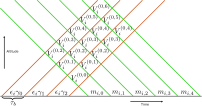
\includegraphics[width=1\linewidth]{code_diagram_modulated.pdf}
	\caption{Range time diagram of the modulated version of the radar code with $S=3$.}
	\label{fig:modulated}
\end{figure}
\begin{equation}
m_{i,w} = \sum_{k=0}^{N-1} \epsilon_{i-k} \sum_{s=0}^{S-1} \gamma_{S-1-s} V^{(k, s + w)}_{i}
\end{equation}
\begin{equation}
d_{i,w} = \sum^{S-1}_{s=0} \gamma_{s} m_{i, s + w}
\end{equation}
\begin{equation}
w \in [0, K - S]
\end{equation}
Where $K$ is the number of bits received.
\begin{equation}
d_{i,w} = \sum_{k=0}^{N-1}\epsilon_{i-k} \sum_{s_1=0}^{S-1} \sum^{S-1}_{s_2=0} \gamma_{s_2} \gamma_{S-1-s_1} V_i^{(k, s_1 + s_2 + w)}
\end{equation}
\begin{equation}
d_{i,w} = \sum_{k=0}^{N-1}\epsilon_{i-k} \sum_{s_1=0}^{S-1} \sum^{S-1}_{s_2=0} \gamma_{s_1} \gamma_{s_2} V_i^{(k, S - 1 - s_1 + s_2 + w)}
\end{equation}
\begin{equation}
d_{i,w} = \sum_{k=0}^{N-1}\epsilon_{i-k}\left[SV_i^{(k, S - 1 + w)}
+ \sum_{s_1=1}^{S-1} \sum^{S-1-s_1}_{s_2=0} \gamma_{s_2} \gamma_{s_1 + s_2} V_i^{(k, S - 1 + s_1 + w)}
+ \sum_{s_1=1}^{S-1} \sum^{S-1-s_1}_{s_2=0} \gamma_{s_2+s_1} \gamma_{s_2} V_i^{(k, S - 1 - s_1 + w)} \right]
\end{equation}
\begin{equation}
A_{s_1} = \sum^{S-1-s_1}_{s_2=0} \gamma_{s_2+s_1} \gamma_{s_2}\text{ for }s_1\in[0, S-1]
\end{equation}
\begin{equation}
d_{i,w} = \sum_{k=0}^{N-1}\epsilon_{i-k}\sum_{s=1-S}^{S-1} A_{|s|} V_i^{(k, S - 1 + s + w)}
\end{equation}
\begin{equation}
\hat{R}^{(h, w)}_\Delta = \frac{1}{L}\sum^{L-1}_{j=0}
\epsilon_{j + \Delta}d_{j + \Delta + h, w}^*
\epsilon_jd_{j + h, w}
\end{equation}
\begin{equation}
\hat{R}^{(h, w)}_\Delta = \frac{1}{L}\sum^{L-1}_{j=0}
\epsilon_{j + \Delta}
\sum_{k_1=0}^{N-1}\epsilon_{j+\Delta+h-k_1}\sum_{s_1=1-S}^{S-1} A_{|s_1|} \left(V_{j+\Delta+h}^{(k_1, S - 1 + s_1 + w)}\right)^*
\epsilon_j
\sum_{k_2=0}^{N-1}\epsilon_{j+h-k_2}\sum_{s_2=1-S}^{S-1} A_{|s_2|} V_{j+h}^{(k_2, S - 1 + s_2 + w)}
\end{equation}
\begin{equation}
\langle \hat{R}^{(h, w)}_\Delta \rangle = \frac{1}{L}\sum^{L-1}_{j=0}
\epsilon_{j + \Delta}
\sum_{k=0}^{N-1}\epsilon_{j+\Delta+h-k}\sum_{s_1=1-S}^{S-1} A_{|s_1|} 
\epsilon_j
\epsilon_{j+h-k}\sum_{s_2=1-S}^{S-1} A_{|s_2|} \left\langle \left(V_{j+\Delta+h}^{(k, S - 1 + s_1 + w)}\right)^* V_{j+h}^{(k, S - 1 + s_2 + w)} \right\rangle
\end{equation}
\begin{equation}
\left\langle \left(V_{j+\Delta+h}^{(k, S - 1 + s_1 + w)}\right)^* V_{j+h}^{(k, S - 1 + s_2 + w)} \right\rangle =
\delta_{s_1, s_2} R_\Delta^{(k, S-1+s_1+w)} +
\delta_{s_1, s_2+1} R_\Delta^{(k, S-1+s_1+w + 0.5)}/2 +
\delta_{s_1, s_2-1} R_\Delta^{(k, S-1+s_1+w - 0.5)}/2
\end{equation}
\begin{equation}
\langle \hat{R}^{(h, w)}_\Delta \rangle =
\sum_{s_1=1-S}^{S-1} A^2_{|s_1|}R_\Delta^{(h, S-1+s_1+w)}+
\frac{1}{2}\sum_{s_1=1-S}^{S-2} A_{|s_1|}A_{|s_1+1|}R_\Delta^{(h, S-1+s_1+w+0.5)}+
\frac{1}{2}\sum_{s_1=2-S}^{S-1} A_{|s_1|}A_{|s_1-1|}R_\Delta^{(h, S-1+s_1+w-0.5)}
\end{equation}
if $\gamma$ is a Barker code we have $A_{|i|}A_{|i+1|}=0$
\begin{equation}
\langle \hat{R}^{(h, w)}_\Delta \rangle =
\sum_{s_1=1-S}^{S-1} A^2_{|s_1|}R_\Delta^{(h, S-1+s_1+w)}
\end{equation}
so we find a biased estimator, where the signal is stronger by a factor
\begin{equation}
\frac{S^2}{S - 1}
\end{equation}
compared to the bias.
one can also deconvolute, to find an exact result.

\subsection{Modulation with fixed code, match filter on pulse}
\begin{equation}
m_{i,w} = \sum_{k=0}^{N-1} \epsilon_{i-k} \sum_{s=0}^{S-1} \gamma_{S-1-s} V^{(k, s + w)}_{i, w}
\end{equation}
\begin{equation}
d_{i,w} = \sum^{S-1}_{s=0} \gamma_{s} m_{i, s + w}
\end{equation}
\begin{equation}
w \in [0, K - S]
\end{equation}
Where $K$ is the number of bits received.
\begin{equation}
d_{i,w} = \sum_{k=0}^{N-1}\epsilon_{i-k} \sum_{s_1=0}^{S-1} \sum^{S-1}_{s_2=0} \gamma_{s_2} \gamma_{S-1-s_1} V_{i,w+s_2}^{(k, s_1 + s_2 + w)}
\end{equation}

\begin{equation}
d_{i,w} = \sum_{k=0}^{N-1}\epsilon_{i-k} \sum_{s_1=0}^{S-1} \sum^{S-1}_{s_2=0} \gamma_{s_1} \gamma_{s_2} V_{i,w+s_2}^{(k, S - 1 - s_1 + s_2 + w)}
\end{equation}
In order to get rid of half overlapping range gates we use
\begin{equation}
V^{(k,s)}_{i,w} = X^{(L, k, s)}_{i,w} + X^{(U, k, s + 1)}_{i,w}
\end{equation}
with
\begin{equation}
\left\langle \left( X^{(z_1, k, s_1)}_{i_1,w_1} \right)^* X^{(z_2, k, s_2)}_{i_2,w_2} \right\rangle = \delta_{s_1,s_2}G^{(z_1, z_2, k, s_1)}_{\Delta, w_1 - w_2}
\end{equation}
with this we have
\begin{align}
\left \langle \left(V_{i_1,w_1+s_2}^{(k, S - 1 - s_1 + s_2 + w_1)} \right)^* V_{i_2,w_2+s_4}^{(k, S - 1 - s_3 + s_4 + w_2)} \right\rangle =\\
G^{(L, L, S-1-s_1+s_2+w_1)}_{\Delta, w_1 - w_2 + s_2 - s_4} \delta_{s_2 - s_1 + w_1, s_4 - s_3 + w_2}\\
+G^{(U, U, S-s_1+s_2+w_1)}_{\Delta, w_1 - w_2 + s_2 - s_4} \delta_{s_2 - s_1 + w_1, s_4 - s_3 + w_2}\\
+G^{(L, U, S-1-s_1+s_2+w_1)}_{\Delta, w_1 - w_2 + s_2 - s_4} \delta_{s_2 - s_1 + w_1, s_4 - s_3 + w_2 + 1}\\
+G^{(U, L, S-s_1+s_2+w_1)}_{\Delta, w_1 - w_2 + s_2 - s_4} \delta_{s_2 - s_1 + w_1 + 1, s_4 - s_3 + w_2}
\end{align}
\begin{align}
\left \langle \left(V_{i_1,w_1}^{(k, s_1)} \right)^* V_{i_2,w_2}^{(k, s_2)} \right\rangle=
\left( G^{(L, L, s_1)}_{\Delta, \delta} + G^{(U, U, s_1 + 1)}_{\Delta, \delta} \right) \delta_{s_1, s_2} + G^{(L, U, s_1)}_{\Delta, \delta} \delta_{s_1, s_2 + 1} + G^{(U, L, s_1 + 1)}_{\Delta, \delta} \delta_{s_1 + 1, s_2}
\end{align}


we see that
\begin{equation}
\left( G^{(z_1, z_2, k, s_1)}_{i, w_1 - w_2} \right)^* = G^{(z_2, z_1, k, s_1)}_{i, w_1 - w_2}
\end{equation}
using this we have
\begin{align}
\left \langle \left(V_{i_1,w_1+s_2}^{(k, S - 1 - s_1 + s_2 + w_1)} \right)^* V_{i_2,w_2+s_4}^{(k, S - 1 - s_3 + s_4 + w_2)} \right\rangle =\\
\left( G^{(U, U, S-s_1+s_2+w_1)}_{\Delta, w_1 - w_2 + s_2 - s_4} + G^{(L, L, S-1-s_1+s_2+w_1)}_{\Delta, w_1 - w_2 + s_2 - s_4} \right) \delta_{s_2 - s_1 + w_1, s_4 - s_3 + w_2}\\
+G^{(L, U, S-1-s_1+s_2+w_1)}_{\Delta, w_1 - w_2 + s_2 - s_4} \delta_{s_2 - s_1 + w_1, s_4 - s_3 + w_2 + 1}\\
+\left( G^{(L, U, S-s_1+s_2+w_1)}_{\Delta, w_1 - w_2 + s_2 - s_4} \right)^* \delta_{s_2 - s_1 + w_1 + 1, s_4 - s_3 + w_2}
\end{align}
\subsection{Modulation with fixed code, decoding first}
\begin{equation}
\langle m_{i_1, w_1}^* m_{i_2, w_2}\rangle = \sum_{s_1=0}^{S-1}\sum_{s_2=0}^{S-1} \gamma_{s_1} \gamma_{s_2} \left\langle \left( V^{(k, S-1-s_1 + w_1)}_{i_1, w_1} \right)^* V^{(k, S-1-s_2 + w_2)}_{i_2, w_2} \right \rangle
\end{equation}

\subsection{Modulation with alternating code}
\begin{equation}
m_{i,w} = \sum_{k=0}^{N-1} \epsilon_{i-k} \sum_{s=0}^{S-1} \gamma^{(k)}_{S-1-s} V^{(k, s + w)}_{i}
\end{equation}
\begin{equation}
\hat{R}^{(h, w)}_\Delta = \frac{1}{L}\sum^{L-1}_{j=0}
\epsilon_{j + \Delta}m_{j + \Delta + h, w}^*
\epsilon_jm_{j + h, w}
\end{equation}

\begin{equation}
\langle \hat{R}^{(h, w)}_\Delta \rangle = \frac{1}{L}
\sum_{s_1=0}^{S-1}
\sum_{s_2=0}^{S-1}
\sum^{L-1}_{j=0}
\sum_{k=0}^{N-1}
\epsilon_{j + \Delta}
\epsilon_{j + \Delta + h - k}\gamma^{(j + \Delta + h - k)}_{S-1-s_1}
\epsilon_j
\epsilon_{i - k} \gamma^{(j + h - k)}_{S-1-s_2}
\langle \left(V^{(k, s_1 + w)}_{j + \Delta + h}\right)^* V^{(k, s_2 + w)}_{j+h} \rangle
\end{equation}


\section{The alternating codes}
\subsection{Short lags expectation value}
\begin{equation}
m^{(c)}_j = \sum_{i=0}^{B-1} \epsilon^{(c)}_i V^{(c)}_{i,j} + \xi^{(c)}_j
\end{equation}
\begin{equation}
\hat{R}^{(h(j_1 - k_1)}_\Delta = \frac{1}{M} \sum_{c=0}^{M-1} \epsilon^{(c)}_{k_1} \epsilon^{(c)}_{k_2} \left(m^{(c)}_{j_1}\right)^* m^{(c)}_{j_2}
\end{equation}
\begin{equation}
\left\langle \hat{R}^{(j_1 - k_1)}_\Delta \right\rangle =
\frac{1}{M} \sum_{c=0}^{M-1} \epsilon^{(c)}_{k_1} \epsilon^{(c)}_{k_2} \left\langle \left(m^{(c)}_{j_1}\right)^* m^{(c)}_{j_2} \right\rangle =
\frac{1}{M} \sum_{i_1=0}^{B-1} \sum_{i_2=0}^{B-1} \sum_{c=0}^{M-1} \epsilon^{(c)}_{k_1} \epsilon^{(c)}_{k_2} \epsilon^{(c)}_{i_1}\epsilon^{(c)}_{i_2} \left\langle \left( V^{(c)}_{i_1,j_1}\right)^* V^{(c)}_{i_2,j_2} \right\rangle
\end{equation}
\begin{equation}
\Delta = k_1 - k_2 = j_1 - j_2 > 0
\end{equation}
\subsection{Long lags expectation value}
\begin{equation}
m^{(c)}_j = \sum_{i=0}^{B-1} \epsilon^{(c)}_i V^{(c)}_{i,j} + \xi^{(c)}_j
\end{equation}
\begin{equation}
\hat{R}^{(h(j_1 - k_1)}_\Delta = \frac{1}{M} \sum_{c=0}^{M-1} \epsilon^{(c)}_{k_1} \epsilon^{(c+1)}_{k_2} \left(m^{(c)}_{j_1}\right)^* m^{(c+1)}_{j_2}
\end{equation}
\begin{equation}
\left\langle \hat{R}^{(j_1 - k_1)}_\Delta \right\rangle =
\frac{1}{M} \sum_{c=0}^{M-1} \epsilon^{(c)}_{k_1} \epsilon^{(c+1)}_{k_2} \left\langle \left(m^{(c)}_{j_1}\right)^* m^{(c+1)}_{j_2} \right\rangle =
\frac{1}{M} \sum_{i_1=0}^{B-1} \sum_{i_2=0}^{B-1} \sum_{c=0}^{M-1} \epsilon^{(c)}_{k_1} \epsilon^{(c+1)}_{k_2} \epsilon^{(c)}_{i_1}\epsilon^{(c+1)}_{i_2} \left\langle \left( V^{(c)}_{i_1,j_1}\right)^* V^{(c+1)}_{i_2,j_2} \right\rangle
\end{equation}
\begin{equation}
\Delta = k_1 - k_2 = j_1 - j_2 > 0
\end{equation}

\subsection{Bias}
the estimator is biased, due to signals coming from higher altitudes, which are caused by the pulse $c-1$
\begin{equation}
\left\langle \hat{R}^{(j_1 - k_1)}_\Delta \right\rangle =
\frac{1}{M} \sum_{i_1=0}^{B-1} \sum_{i_2=0}^{B-1} \sum_{c=0}^{M-1} \epsilon^{(c)}_{k_1} \epsilon^{(c)}_{k_2} \epsilon^{(c-1)}_{i_1}\epsilon^{(c-1)}_{i_2} \left\langle \left( V^{(c-1, 1)}_{i_1,j_1}\right)^* V^{(c-1, 1)}_{i_2,j_2} \right\rangle
\end{equation}
SPECULATION: as the product of codes is random, we do not expect constant $1$ but $0$ with standard deviation of $1/\sqrt{B}$ for all indices for which the expectation value is not zero.
the additional (implicit) averaging over $B$ will contribute another factor $1/\sqrt{B}$

\subsection{Variance}
\begin{equation}
\left\langle \left| \hat{R}^{(j_1 - k_1)}_\Delta \right|^2 \right\rangle =
\frac{1}{M^2} \sum_{c_1=0}^{M-1} \sum_{c_2=0}^{M-1}
\epsilon^{(c_1)}_{k_1} \epsilon^{(c_1)}_{k_2}
\epsilon^{(c_2)}_{k_1} \epsilon^{(c_2)}_{k_2}
\left\langle
m^{(c_1)}_{j_1} \left( m^{(c_1)}_{j_2}\right)^*
\left(m^{(c_2)}_{j_1}\right)^* m^{(c_2)}_{j_2}
\right\rangle
\end{equation}
\begin{equation}
\mathrm{Var}\left[\hat{R}^{(j_1 - k_1)}_\Delta \right] =
\frac{1}{M^2} \sum_{c_1=0}^{M-1} \sum_{c_2=0}^{M-1}
\epsilon^{(c_1)}_{k_1} \epsilon^{(c_1)}_{k_2}
\epsilon^{(c_2)}_{k_1} \epsilon^{(c_2)}_{k_2}
\left\langle m^{(c_1)}_{j_1} \left(m^{(c_2)}_{j_1}\right)^* \right\rangle
\left\langle \left(m^{(c_1)}_{j_2}\right)^* m^{(c_2)}_{j_2} \right\rangle
\end{equation}
\begin{equation}
\mathrm{Var}\left[\hat{R}^{(j_1 - k_1)}_\Delta \right] \approx \frac{1}{M}
\left\langle m^{(c)}_{j_1} \left(m^{(c)}_{j_1}\right)^* \right\rangle
\left\langle \left(m^{(c)}_{j_2}\right)^* m^{(c)}_{j_2} \right\rangle
\end{equation}
\begin{equation}
\left\langle \left(m^{(c)}_j\right)^* m^{(c)}_j \right\rangle = \sum_{i_1=0}^{B-1} \sum_{i_2=0}^{B-1} \epsilon^{(c)}_{i_1} \epsilon^{(c)}_{i_2} \left\langle V^{(c)}_{i_1,j}\left(V^{(c)}_{i_2,j}\right)^*\right\rangle + P_n \approx BP + P_n
\end{equation}
\begin{equation}
\mathrm{Var}\left[\hat{R}^{(j_1 - k_1)}_\Delta \right] = \frac{(BP + P_n)^2}{M}
\end{equation}






\section{Hypothesis on code length}
\section{Code with cyclic difference set for $\tau_i$}
\section{Simulation}
\subsection{Monte Carlo Generation}
The most straight-forward approach to generate random numbers following a wide-sense stationary process is as follows:
\begin{equation}
R^{(h)}_{jk} = \langle (V_{j}^{(h)})^* V_k^{(h)} \rangle
\end{equation}
where $R^{(h)}_{jk}$ is interpreted (for some fixed $h$) as a correlation matrix for the random vector $V_{j}^{(h)}$ which is to be generated.
We can satisfy the correlation properties by a linear transformation
\begin{equation}
V_j^{(h)} = \sum_{i} T_{ji}f_i
\end{equation}
where $T_{ji}$ must be of toeplitz type and $f_i$ are uncorrelated standard normal Gaussian circular-symmetric random variables with $\langle f_i f_j \rangle = \delta_{ij}$.
This yields
\begin{equation}
R^{(h)}_{jk} = \sum_{i,l} \langle (T_{ji}f_i)^* T_{kl}f_l \rangle = \sum_{i} T_{ji}^* T_{ki}.
\end{equation}
Using that the matrix $T$ is symmetric and seeing that $R^{(h)}_{jk}$ must be positive semidefinite (as it is a covariance matrix) we can calculate $T$ with some square root of matrix algorithm.\\
However all of this can be done more efficiently by using the time stationary of the process.
Note that $T$ is of toeplitz type simply means that we actually need a convolution of $f$ with $T$ where $T$ must be symmetric with a length of at least $2M + 1$ so that the points up to $M + 1$ can be correlated.
However, the generated time series would not have the true correlation properties of the ACF if it is truncated after $M+1$.
The ACF can be either truncated after $n-1$, where $n$ is the total length of the time series, or when the ACF approaches approximately zero.
Now, denote the length of the ACF by $K$.
The convolution is given by
\begin{equation}
V_j^{(h)} = \sum_{i=1-K}^{K-1} T_{i}f_{j - i}.
\end{equation}
It follows that,
\begin{equation}
R^{(h)}_{jk} = \langle (V_{j}^{(h)})^* V_k^{(h)} \rangle = \sum_{l=1-K}^{K-1} \sum_{m=1 - K}^{K-1} T_{l} T_{m} \langle f_{j - l} f_{k - m} \rangle.
\end{equation}
Using that $\langle f_{j - l} f_{k - m} \rangle = \delta_{m, k - j + l}$ and substituting $\Delta=j-k$ yields
\begin{equation}
R^{(h)}_\Delta = \sum_{i=1-K}^{K-1} T_{i} T_{i - \Delta}
\end{equation}
where it is assumed that $T$ is zero padded for all indices which fall out of range.
Applying a Fourier transform over $\Delta$ on both sides results in
\begin{equation}
\mathrm{DCT}[R^{(h)}]_j = \sum_{i=1-K}^{K-1} T_{i}\mathrm{DTFT}[T_{i - \Delta}]_j.
\end{equation}
From the definition of the $\mathrm{DTFT}$ follows that
\begin{equation}
\mathrm{DCT}[R^{(h)}]_j = \sum_{l=1-K}^{K-1} T_{l}\exp\left(\frac{i2\pi lj}{2K-1} \right) \mathrm{DCT}[T]_j,
\end{equation}
using the definition of the Fourier transform again results in
\begin{equation}
\mathrm{DCT}[R^{(h)}]_j = (2K - 1)\left( \mathrm{DCT}[T]_j \right)^2.
\end{equation}
Now there are two options: Either one solves for $T$ and does the convolution in the time domain, or one solves for the Fourier transform of $T$ and does the convolution in Fourier space.
Which one is faster depends on the choice of $K$.
The first approach is preferred when $K$ is fixed which results in an asymptotic runtime of $\mathcal{O}(Kn)$.
In the case $K=n$ latter approach is preferred as it results in a runtime of $\mathcal{O}(n\log(n))$.
However, choosing $K=n$ has not a real practical use case, as the ACF can always be cut off at small value, in the sense that $M \gtrsim K$.

\subsection{Discrete Fourier and Cosine Transform}
We define the Discrete Time Fourier Transform as
\begin{equation}
\mathrm{DTFT}[x]_n = \sum^{N-1}_{k=0} x_k \exp\left(-\frac{i2\pi kn}{N}\right)
\end{equation}
and its inverse by
\begin{equation}
\mathrm{DTFT}^{-1}[x]_n = \frac{1}{N}\sum^{N-1}_{k=0} x_k \exp\left(\frac{i2\pi kn}{N}\right).
\end{equation}
Sometimes, it can be handy to allow negative indices for a more ``natural'' representation.
In the case that $n$ is even
\begin{equation}
\mathrm{DTFT}^{-1}[\hat{x}]_n = \frac{1}{N}\sum^{N/2+1}_{k=-N/2+2} \hat{x}_k \exp\left(\frac{i2\pi kn}{N}\right)
\end{equation}
and in the uneven case
\begin{equation}
\mathrm{DTFT}^{-1}[\hat{x}]_n = \frac{1}{N}\sum^{(N-1)/2}_{k=-(N-1)/2} \hat{x}_k \exp\left(\frac{i2\pi kn}{N}\right).
\end{equation}
The Discrete Cosine Transform of Type I is defined as
\begin{equation}
\mathrm{DCT}[x']_n = x'_0 + x'_{N'-1}(-1)^n + 2\sum_{k=0}^{N'-1} x'_k \cos \left(\frac{\pi k n}{N'-1}  \right).
\end{equation}
and its inverse is given by
\begin{equation}
\mathrm{DCT}^{-1}[x']_n = \frac{\mathrm{DCT}[x']_n}{2(N'-1)}
\end{equation}
The $\mathrm{DCT}$ is equivalent to a $\mathrm{DTFT}$ for a symmetric input but it is faster and uses less memory.
More precisely, it can be shown that for $N=2(N'-1)$ and $x_i=x'_i$ for $i\in[0, N'-1]$ and $x_i=x'_{N-i}$ for $i\in[N', N-1]$ that
\begin{equation}
\mathrm{DTFT}^{-1}[x]_n = \mathrm{DCT}^{-1}[x']_n 
\end{equation}
where $n\in[0, N'-1]$.
\subsection{From the continuous Fourier transform to the DCT}
\begin{align}
R(\tau) &= \int_{-\infty}^{\infty} \exp(-2\pi i\omega\tau) S(\omega) \d \omega \\
&=2\int_{0}^{\infty} \cos(2\pi i\omega\tau) S(\omega) \d \omega
\end{align}
\begin{align}
S(j\Delta_\omega) &= S_j\\
R(j\Delta_\tau) &= R_j
\end{align}
As we only store a fixed number of samples, the period must be finite.
This means, that a periodic continuation beyond the last sample ($S_{N-1}$) must be specified.
In our case, even symmetry around $N-1$ is considered.
As the first and last sample's bins shall be centered around $\omega=0$ and $\omega=(N-1)\Delta_\omega$ respectively, they have half width, so the integral becomes
\begin{align}
R_k = S_0\Delta_\omega + \cos({2\pi (N-1) k\Delta_\omega \Delta_\tau}) S_{N-1} + 2\sum_{j=1}^{j=N-2}\cos({2\pi j k \Delta_\omega \Delta_\tau}) S_j \Delta_\omega 
\end{align}
The maximum frequency (half bandwidth in our case) is $B = \Delta_\omega (N - 1)$.
Now we can use the sampling theorem to find $\Delta_\tau = 1/(2B)$.
\begin{align}
R_k = \left(S_0 + (-1)^kS_{N-1} + 2\sum_{j=1}^{j=N-2}\cos \left(\frac{\pi j k}{N-1}  \right) S_j \right) \Delta_\omega
\end{align}
This is a type I DCT (Discrete Cosine Transform) according to scipy definition. 

\section{A lower bound for the variance}

Assumptions made: monostatic radar, binary coded transmission, gaussian process
A lower bound for the variance of any ACF estimation independent of the estimator is to be calculate, by means of the Cramér–Rao bound.
What the radar measures (independent of the estimator) is
\begin{equation}
m_i=\sum_{k=0}^{N-1} \epsilon_{i-k} V^{(k)}_i.
\end{equation}
The parameters to be estimated are 
\begin{equation}
R^{(k)}_\Delta=\langle (V_{j+\Delta}^{(k)})^* V_j^{(k)} \rangle.
\end{equation}
The individual $m_i$ are random Gaussian distributed.
The information is contained in the correlations.
Define the probability density function $P = P(m_{1..n}, R^{(0..N-1)}_{1..M})$.
We need to calculate $P$.
the random variables $V^{(k)}_i$ are normally distributed with a correlation matrix of toeplitz type given by
\begin{equation}
\Sigma^{(k)}_{ij} = R_{i-j}^{(k)}
\end{equation}
then $m_i$ are Gaussian distributed according to
\begin{equation}
\Sigma_{ij} = \sum_{k=0}^{N-1} \epsilon_{i-k} \epsilon_{j-k} R_{|i-j|}^{(k)}.
\end{equation}
we note that the matrix is periodic with $\Sigma_{i,j} = \Sigma_{i+L,j+L}$
where we imagine the matrix to be infinite in size as the auto correlation never drops to precisely to zero.
The fisher information matrix for any zero mean Gaussian is
\begin{equation}
\mathcal{I}_{ij} = \frac{1}{2}\mathrm{tr}\left(\Sigma^{-1} \frac{\partial \Sigma}{\partial \theta_i} \Sigma^{-1} \frac{\partial \Sigma}{\partial \theta_j} \right)
\end{equation}
where each $\theta_i$ identifies exactly one parameter $\theta_i = R^{(k_i)}_{\Delta_i}$
\begin{equation}
\frac{\partial \Sigma_{ij}}{\partial \theta_p} = \epsilon_{i - k_p}\epsilon_{j - k_p}\delta_{|i-j|,\Delta_p}
\end{equation}
the fisher information matrix is
\begin{equation}
\mathcal{I}_{ij} = \frac{1}{2}\sum_{k_1, k_2, k_3, k_4}
\Sigma^{-1}_{k_1, k_2}
\epsilon_{k_2 - k_i}\epsilon_{k_3 - k_i}\delta_{|k_2-k_3|,\Delta_i}
\Sigma^{-1}_{k_3, k_4}
\epsilon_{k_4 - k_j}\epsilon_{k_1 - k_j}\delta_{|k_4-k_1|,\Delta_j}
\end{equation}
defining
\begin{equation}
\sigma_{\Delta_1, \Delta_2} =
\epsilon_{k_2 - k_i}\epsilon_{k_2 + \Delta_1 - k_i}
\epsilon_{k_1 - k_j}\epsilon_{k_1 + \Delta_2 - k_j}
\Sigma^{-1}_{k_1, k_2}
\Sigma^{-1}_{k_2 + \Delta_1, k_1 + \Delta_2}
\end{equation}
swapping $k_1 \leftrightarrow k_2$ and using symmetry of $\Sigma^{-1}$ it can be shown that
\begin{equation}
\sigma_{\Delta_1, \Delta_2} =
\epsilon_{k_1 - k_i}\epsilon_{k_1 + \Delta_1 - k_i}
\epsilon_{k_2 - k_j}\epsilon_{k_2 + \Delta_2 - k_j}
\Sigma^{-1}_{k_1, k_2}
\Sigma^{-1}_{k_1 + \Delta_1, k_2 + \Delta_2}
\end{equation}
using this definition results in
\begin{equation}
\mathcal{I}_{ij} = \frac{1}{2}\sum_{k_1, k_2}
\left[\sigma_{\Delta_i, \Delta_j}+\sigma_{-\Delta_i, \Delta_j}+
\sigma_{\Delta_i, -\Delta_j}+\sigma_{-\Delta_i, -\Delta_j}\right]
\end{equation}
for an infinite length random code with high $N$ the diagonal elements of $\Sigma$ grow proportional to $N$, while the off-diagonal elements have zero expectation value.
They do have a standard deviation of $\sqrt{N}$ but for sufficient large $N$ a diagonal matrix is found:
\begin{equation}
\Sigma_{ij} = \delta_{ij} \sum_{k=0}^{N-1} R_{0}^{(k)}
\end{equation}
which has the trivial inverse
\begin{equation}
\Sigma^{-1}_{ij} = \delta_{ij} \left(\sum_{k=0}^{N-1} R_{0}^{(k)}\right)^{-1}
\end{equation}
when substituting this into $\sigma$ it can be seen that $\Delta_i=\Delta_j$ and $k_1=k_2$ must hold for $\sigma \neq 0$.
\begin{equation}
\sigma_{\Delta_1, \Delta_2} = \delta_{k_1 k_2}\delta_{\Delta_1\Delta_2}
\epsilon_{k_1 - k_i}\epsilon_{k_1 + \Delta_1 - k_i}
\epsilon_{k_2 - k_j}\epsilon_{k_2 + \Delta_2 - k_j}
\left(\sum_{k=0}^{N-1} R_{0}^{(k)}\right)^{-2}
\end{equation}
the epsilons will square away for $k_i=k_j$ or special cases like $\Delta_1 = \Delta_2 = k_j, k_i=0$ but we are only interested in the main diagonal of the fisher matrix, so $k_i=k_j$.
the fisher matrix is thus approximately given by
\begin{equation}
\mathcal{I}_{ij} = \delta_{ij} L \left(\sum_{k=0}^{N-1} R_{0}^{(k)}\right)^{-2}
\end{equation}
where we assumed $L$ measurements 

so the lower bound for the standard deviation is
\begin{equation}
\sigma \geq \frac{1}{\sqrt{L}}\sum_{k=0}^{N-1} R_{0}^{(k)}
\end{equation}


\section{Calculation of codes}

Due to technical limitations of the radar we have $\epsilon_i \in [-1, 1]$ and a naive brute force algorithm finds the following (shortest) codes for a given $N$ and $M$
\begin{center}
	\centering
	\begin{tabular}{cccc}
		\toprule
		$L$&$N$&$M$&Code\\
		\midrule
		24&5&4&$-+-+++++++-++--+-++-+++-$\\
		32&6&5&$-++-++++++++---++---+----++-+---$\\
		32&8&3&$-+--++++++++-+---+--++++--+++---$\\
		40&7&4&$-+--+++++++++-+++--+-+++----+-+++--++++-$\\
		48&8&5&$--++++++++-+-+--+--+-++--+---+----++---++-+----+$\\
		\bottomrule
	\end{tabular}
\end{center}
Note that we have used that every code which is valid for $w$ is also valid for $-w$, because the value of the sum does not change if the code is shifted by $w$, due to the codes periodicity.


\section{Possibility of using a Quantum SAT-Solver}

The condition could be transformed to a boolean SAT problem, which could be solved by Grover's algorithm on a quantum computer.
See \url{https://learn.qiskit.org/course/introduction/grovers-search-algorithm}.
However, there are also different SAT-Solvers, which might pose a speedup compared to random guessing.
There are also combinations of improved SAT-Solvers and quantum; investigate this.


\end{document}








